\documentclass[oneside,12pt]{report}  

% the dimensions of the page
\textheight=9.25in \topmargin=-0.5in   %See note in Chapter 8 of Sample Report about "Page scaling" option in Adobe
\textwidth=6.0in
\oddsidemargin=0.3in
\evensidemargin=0.3in  % Needed to balance even and odd pages in twoside print copy


% Useful packages
\usepackage{dtklogos}
\usepackage [font=small, labelfont=bf]{caption}
\usepackage{amsmath}
\usepackage{bm}
%\usepackage[colorlinks=true,pagebackref,linkcolor=blue]{hyperref}
\usepackage{amsfonts}
\usepackage{amsthm}
\usepackage{amsmath}
\usepackage{algorithm}
\usepackage{algorithmic}
\usepackage{graphicx, subfigure}
\usepackage{caption}
\usepackage{excludeonly}
\usepackage{url}
\usepackage{graphicx}
\graphicspath{{./extra/}} 

%\usepackage{doc}
%% Following sets up logic and formatting for conditional twoside copying
%\usepackage{ifthen, color, fancyvrb}
%\usepackage{nextpage}\pagestyle{plain}
%\newcommand\myclearpage{\cleartooddpage
%  [\thispagestyle{empty}]
%  }

\DeclareMathOperator*{\argmin}{arg\ min}
\DeclareMathOperator*{\sign}{sign}

% Note special alternative codes for using TWO bibliographies; see cautionary note in
\DeclareGraphicsExtensions{ps,eps,PNG,png}

% Theorem-like command definitions:
\newtheorem{theorem}{Theorem}[chapter]
\newtheorem{lemma}{Lemma}[chapter]
\newtheorem{definition}{Definition}  % Note, this italicizes everything

% Print the chapter and sections in the toc
\setcounter{tocdepth}{1}

% Specify which files to typeset for this run (note that overall pagination is preserved)
%\includeonly{chapter1, chapter2}
% Specify which files NOT to typeset for this run (note that overall pagination is preserved)
%\excludeonly{}

% Groundwork for allowing double-sided copying with blank versos
\def\prefacesection#1{
\chapter*{#1}
\addcontentsline{toc}{chapter}{#1}
}

\begin{document}


\def\thefootnote{\fnsymbol{footnote}}

\thispagestyle{empty}

% The numbers below controls the amount of space between the following sections
\def\shiftdowna{0.32in}  % Adjust for balance
\def\shiftdownb{0.22in}  % Adjust for balance

% Set up the boiler plate at the top of the page

\begin{center}
\textbf{{\large Mathematical Modeling and Consulting }}\\

\vspace \shiftdowna
%
\includegraphics[width=0.5\textwidth]{jhu.png}\\

\includegraphics[width=2.5in]{BJU.jpg}\\

% Home Department
\vspace \shiftdowna
\underline {Sponsor}\\ 
\vspace{5pt}
\textbf{\large Blue Jays Unlimited} \\
\vspace\shiftdowna
\textbf{{Final Report}}

% TITLE
\vspace \shiftdowna
\textbf{{\Large Modeling and Simulating Fan Participation at Large Scale Sporting Events}}

% STUDENTS
\vspace{0.35in}
\underline {Team Members}\\
\vspace{5pt}
Ahmed Aly, Department of Biomedical Engineering\\
\texttt{aaly2@jhu.edu} \\
\vspace{5pt}
Steven Su, Department of Biomedical Engineering\\
\texttt{ssu7@jhu.edu} \\
\vspace{5pt}
Danni Tang, Department of Biomedical Engineering\\
\texttt{danni@jhu.edu} \\
%\vspace{10pt}
%Jane Doe (Report Coordinator), Home Department
%%\texttt{jane.doe@jhu.edu}

% INSTRUCTOR
\vspace \shiftdownb
\underline {Academic Mentor} \\
\vspace{5pt}
\text{Dr.~N.~H.~Lee}, Applied Mathematics and Statistics\\
\texttt{nhlee@jhu.edu}

%% Consultants
%\vspace \shiftdownb 
%\underline {Consultant}\\
%\vspace{5pt}
%Jason Bourne\\

% DATE
\vspace \shiftdowna
Date: Last Compiled on \today

\end{center}

\vfill  %Fill page to force following note to bottom
\footnoterule
\noindent \small{This project is fictionally supported by Blue Jays Unlimited.}

% Begin ABSTRACT
\ifthenelse{\boolean{@twoside}}{\myclearpage}{}
\prefacesection{Abstract}
\paragraph{}
Having a loud and supportive home crowd is the ultimate home team advantage for any sports team. This is especially true for collegiate sports. In this work we developed a simple stochastic model for modeling cheering in crowds at large sporting events. Our model accounts for differences in innate support level for a sports team between fans as well as the number and length of time surrounding fans have been cheering. It uses these factors to predict whether a single fan will start to cheer and then simulates over time how cheering in a crowd progresses. The results from the model are promising: cheering in a crowd can either increase greatly or increase slightly, depending on how the parameters of the model are varied. 

% Begin ACKNOWLEDGMENTS
\ifthenelse{\boolean{@twoside}}{\myclearpage}{}
\prefacesection{Acknowledgments}
\paragraph{}
We would like to thank Blue Jays Unlimited for fictionally sponsoring us. In addition, we appreciate the unwavering support and patient guidance our academic mentor, Dr.~Nam H.~Lee, has given us. We would also like to thank our classmates for their support. 

% Table of contents, List of Figures, and List of Tables.
\ifthenelse{\boolean{@twoside}}{\myclearpage}{}
\tableofcontents

\ifthenelse{\boolean{@twoside}}{\myclearpage}{}
\listoffigures

\ifthenelse{\boolean{@twoside}}{\myclearpage}{}
\listoftables

%\ifthenelse{\boolean{@twoside}}{\myclearpage}{}
%\listoftables


\renewcommand{\thefootnote}{\arabic{footnote}}
\setcounter{footnote}{0}

\ifthenelse{\boolean{@twoside}}{\myclearpage}{}
\prefacesection{Introduction}
\paragraph{}
A loud and supportive home crowd is the ultimate home team advantage for any sports team. Past research has shown that the home crowd advantage can have a profound effect on deciding who wins a sporting event \cite{Jamieson_2010}. Across all major professional sporting leagues in the United States, the home team at any sporting event wins approximately 60\% of the time, a statistically significantly higher winning percentage then the expected 50\% \cite{Jamieson_2010}. The home crowd advantage is even more profound in college athletics. Studies have shown that in certain collegiate sports, the home team wins up to 66\% of the games played \cite{Snyder_1985}.

\paragraph{}
In addition to helping the home team win, a loud and supportive home crowd can also improve the ambiance of a sporting event. Whether fans are chanting the school fight song, waving a rally towel, doing the wave, or clapping in general applause, the fans are not only showing support for the home team but also enhancing the general atmosphere of the sporting event at the same time. Note that all of these actions will hence be collectively termed ``cheering.'' For this and previously stated reasons, it is evident that cheering is essential at collegiate sporting events. Cheering improves the collegiate sporting experience for both the athletic teams as well as the fans. 

\paragraph{}
The Johns Hopkins University, located in Baltimore, MD, has a proud athletic tradition to go along with its long standing reputation for strong academics. The Johns Hopkins University Blue Jays have amassed 47 national championships and 187 conference titles \cite{hopathletic}. The Blue Jays have excelled at many sports including Men's Lacrosse, Men's Swimming, Men's Football, and Men's Baseball. The Men's Lacrosse team has won 44 national championships, most recently in 2007, while the Men's Swimming team won 32 conference championships, including an astounding streak of 28 consecutive conference championships from 1971-1998 \cite{hopathletic}. More recently, the Men's Football and Baseball teams were each conference champions for three consecutive years from 2009 through 2011 \cite{hopathletic}. As with any collegiate athletic program, The Johns Hopkins University and its supporters are always looking for ways to improve its athletic teams' performances so that they may continue in their winning ways.

\ifthenelse{\boolean{@twoside}}{\myclearpage}{}
\prefacesection{Background}
\paragraph{} 
Blue Jays Unlimited (BJU), established in 1995, is a volunteer group of alumni, friends and staff dedicated to supporting and promoting Johns Hopkins athletics \cite{bjuwebsite}. BJU is the official booster club for Johns Hopkins athletics and has more than 3000 active members, who have raised more than \$4 million in funds to improve the Johns Hopkins athletic experience for both student athletes and fans alike \cite{bjuwebsite}. These funds provide money for capital projects as well as scholarship and operational endowments \cite{bjuwebsite}. Past BJU projects have included renovations of the Newton H.~White Athletic Center as well as recognition banners for championship teams \cite{bjuwebsite}.

\paragraph{}
BJU is present at nearly all major Johns Hopkins sporting events to encourage fans to support their Blue Jays in a vociferous and family-friendly manner to propel their Hopkins' teams to victory. It is their goal to provide Johns Hopkins' athletic teams with a spirited home crowd to cheer them on. As such, BJU is interested in maximizing the amount of fan participation in cheering at sporting events held on Homewood Field at the Homewood campus of The Johns Hopkins University. More specifically, they believe that they can increase fan participation in cheering events by strategically placing ``cheer starters'' in the home crowd to encourage other fans to participate in cheering. Cheer starters are student volunteers who lead and urge other fans around them to cheer.

\begin{figure}[h]
	\begin{center}
			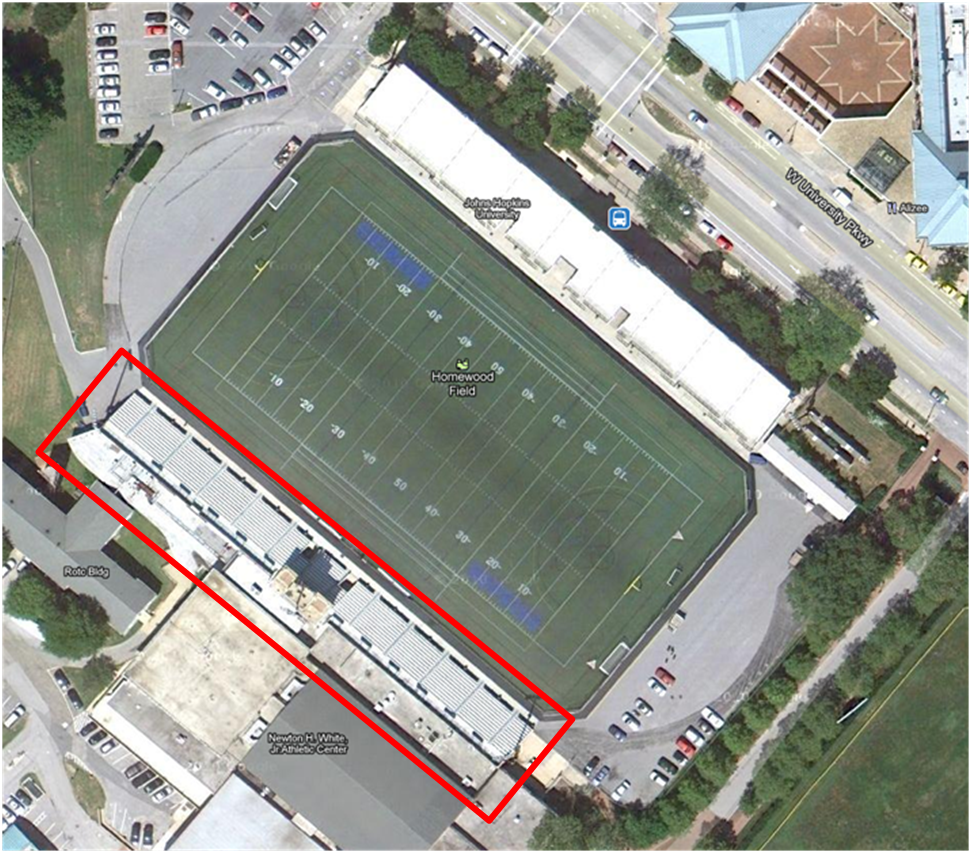
\includegraphics[height=2.25in] {Bleachers.png}
	\end{center}
	\caption[Homewood Field located on the Homewood campus of The Johns Hopkins University in Baltimore, MD.]{Homewood Field located on the Homewood campus of The Johns Hopkins University in Baltimore, MD. The bleachers in the lower left corner outlined in red are traditionally reserved for home team fans.}
	\label{fig:homewoodfield}
\end{figure}

\paragraph{}
Consider the satellite image of Homewood Field in Figure \ref{fig:homewoodfield}, courtesy of Google Maps. Homewood Field's capacity is approximately 8500 spectators \cite{wiki}. The long rectangular section of bleachers outlined in red in the lower left of portion of the image seats approximately 4000 fans and is traditionally reserved for Blue Jays' fans. For nearly all major Hopkins' sporting events, these home team bleachers are filled to capacity. As such, BJU is specifically interested in maximizing fan cheering in these home team bleachers. 

\ifthenelse{\boolean{@twoside}}{\myclearpage}{}
\prefacesection{Problem Statement and Objectives}
{\bf{\Large Problem Statement}}
\paragraph{}
BJU wants to know if cheer starters can actually increase cheering and also wants a simple model of fan participation in cheering in the home team bleachers on Homewood Field.
\newline
\newline
{\bf{\Large Objectives}}
\paragraph{}
Our task is to provide BJU with a simple model of fan participation in cheering at Homewood Field in the home team bleachers as well as simulation results from the model which determine if their belief about cheer starters is accurate.
\ifthenelse{\boolean{@twoside}}{\myclearpage}{}
\prefacesection{Analysis}
Because this model is a simulation, it is imperative to clearly define simplifications and assumptions we have made in the model.
\paragraph{Simplifications and Assumptions}
	\begin{itemize}
	\item The willingness of a fan in a crowd to cheer depends on the number of people cheering around the given fan as well as how long the surrounding people have been cheering. The greater the number of people surrounding a fan who are cheering, and the longer the surrounding people have been cheering, the more likely that fan will start to cheer.
	\item The innate support level a fan has for the team also influences the willingness of that fan to start cheering.
	\item Once a fan starts to cheer, he/she continues cheering until the end of the simulation.
	\item The performance of the sports team does NOT influence cheering.
	\end{itemize}

%\paragraph {Simplifications and Assumptions}
%
%The stimulus in this case would be the performance of the team. For the purpose of simplicity we will assume that the stimulus is average. From there, we can take a snap shot of the crowd's behavior and ignore the dependence of cheering on the team's performance. Each snap shot can be represented by a "round".  
%\newline
%For the internal state of the individual we can assign base "cheer number" using a stochastic process. We will simplify cheering as a probabilistic switch with a universal threshold that if exceeded the individual will be considered cheering otherwise the indivdual will not be cheering. This will simplify the problem because it will allow us to ignore the continuos gradient and different levels of cheering. 
%\newline
%We will simplify the relationship of the willingness to cheer and the surrounding individuals to only include the individuals that are directly surrounding the intended member.

\paragraph {Computational Simulation}
\paragraph{}
Using MATLAB, we start by generating an arbitrary sized $n$ x $m$ matrix, $X$, to represent a $nm$ sized crowd. The number of rows, $n$, and columns, $m$, can be changed based on the user's liking. However, for our purposes we are choosing to make $X$ a long rectangular matrix to imitate the physical dimensions of the home team bleachers on Homewood Field. The matrix $X$ represents a crowd and each element in it corresponds to a specific fan in the crowd. For example $X_{ij}$ represents fan $ij$. Each element in $X$ is filled with the corresponding fan's innate support level for the team. Each fan's innate support level was generated by sampling from a normal random distribution with a mean of 10 and a standard deviation of 1 as shown in (\ref{1}). 

\begin{equation}
X_{ij}\sim Norm(10,1),~\forall~i\in[1,n],~j\in[1,m].
\label{1}
\end{equation}

\paragraph{}
A normal distribution fits the distribution of innate support levels that a crowd of fans has very well in the following ways. The majority of fans who attend sporting events are average or close to average fans; they will cheer if others around them cheer for a long enough time \cite{DI2003}. A smaller proportion are super fans who will cheer regardless of what anyone else around them is doing \cite{DI2003}. A smaller proportion of attendees may also be less supportive of the team; they require a greater amount of encouragement to start cheering than the average fan \cite{DI2003}. This is well represented in a normal distribution where most of the distribution is centered around the mean and an increasingly smaller proportion of the distribution is found moving away from the mean in both directions \cite{DI2003}. In this model the mean was set to 10 and the standard deviation was set to 1 to ensure that it was highly unlikely that a fan was assigned a negative innate support level. (i.e.~it is very unlikely to sample a number from the normal distribution that is more than 10 standard deviations from the mean.) This makes the math much easier when considering the dependence on the surrounding people, as it will be shown later.

\paragraph{}
Next, we set an initial threshold, $T_{init}$. The initial threshold is used to determine which of the fans in the matrix are \textit{initially} cheering. Another $n$ x $m$ matrix, $X'$, was then created. (Note that $X'$ does NOT denote the transpose of matrix X. $X'$ is an seperate matrix.) Each element in $X'$ is initially assigned a value of 1, if the corresponding element in $X$ (i.e.~the element in $X$ with the same row and column indices) had a value which was greater than or equal to the initial threshold, otherwise the element is given a value of 0. See (\ref{2}). $X'$ is the matrix used to keep track of who is cheering. A value of 1 in $X'$ means that given fan is cheering, while a value of 0 means that given fan is not cheering. 

\begin{equation}
X'_{ij}=1~if~X_{ij}\geq T_{init},~X'_{ij}=0~if~X_{ij}<T_{init}.
\label{2}
\end{equation}

\paragraph{}
Any fan with an innate support level greater than 1 standard deviation above the mean is far above the average fan and can be considered a super fan who would be initially cheering. As such, $T_{init}$ was appropriately set to equal 11, which is 1 standard deviation above the mean of the normal distribution used to generate the innate support levels.

\paragraph{}
As previously stated, whether a fan starts to cheer depends on how many directly adjacent fans around the given fan are cheering, as well as the length of time those fans have been cheering. $S$ is a $n$ x $m$ matrix which stores how many people surrounding a given fan are cheering at a given time. Each element in $S$ has corresponding elements with the same row and column indices in both $X$ and $X'$, all of which store different model values for the same individual fan. We define a round, $r$, to be the passing of an arbitrary time interval (approximately 3-5 seconds, in this case). We then create a fourth $n$ x $m$ matrix, $Y$, and compute the individual elements of $Y$ according to (\ref{3}). 

\begin{equation}
Y_{ij}=X_{ij}(S_{ij})+r,~\forall~i\in[1,n],~j\in[1,m].
\label{3}
\end{equation}

Again, each element in $Y$ represents an individual fan and has corresponding elements in $X$, $X'$, and $S$, with the same row and column indices. We then compare each of the elements in $Y$ to an absolute threshold, $T_{absolute}$. If an individual's score in $Y$ is greater than or equal to the absolute threshold, the individual will begin to cheer, and we set the corresponding element in $X'$ equal to 1. This is shown in (\ref{4}). If the individual's score in $Y$ is less than the absolute threshold, we do nothing to the corresponding element in $X'$ (i.e.~it remains 0).  

\begin{equation}
X'_{ij}=1~if~Y_{ij}\geq T_{absolute}.
\label{4}
\end{equation}

\paragraph{}
We repeat this process for each round (i.e.~compute $Y$, update $X'$ based on the new $Y$, and then update $S$ for the next round based on the new $X'$) until we reach the desired number of rounds, $R$. During each round, we take snapshots of the crowds by storing $X'$ for that round. By doing so, we can compare $X'$ between the rounds and also compute the percentage of fans who are cheering in each round. It is important to note, by computing $Y$ as shown in (\ref{3}), the likelihood of a fan starting to cheer increases with the number of surrounding fans who are cheering (i.e.~as $S_{ij}$ increases) and also increases with the length of time those fans have been cheering (i.e.~as $r$ increases).

\paragraph{}
To test the effect of the number of cheer starters, we randomly place $CS$ number of cheer starters in the crowd. To implement the $CS$ cheer starters into the model, when we initialize $X'$ we randomly choose $CS$ distinct row and column indices in $X'$ and assign those elements to equal 1. By doing this, we insure that the $CS$ cheer starters are initially cheering and remain cheering for the entire simulation. The crowd simulation was then run and the final percentage of cheering fans after 10 rounds was computed as previously described. We repeated this 1000 times for the given $CS$ value and for each of the 1000 trials we recorded the final percentage of cheering fans after the 10 rounds. We then averaged these percentages over all 1000 trials to come up with the average final percentage of cheering fans for that given $CS$ value. We repeated this Monte Carlo procedure for all $CS$ values in the range of $1 \leq CS \leq 50$. The average final percentage of cheering fans for each $CS$ value was then compared to the average final percentage of cheering fans when there were zero cheer starters, using a simple t-test.

\paragraph{Final Parameter Values}
\paragraph{}
Due to computational limits, we could not simulate a crowd of 4000 fans. Instead we downsized our crowd size to 2000 fans and choose to simulate a crowd of 20 by 100 fans. The matrix produced by simulating 20 by 100 fans is long and rectangular and thus similar in shape to the home team bleachers at Homewood Field. We decided to do 10 rounds per simulation. 
\paragraph{}
For the threshold values, we decided to set our initial threshold at 11 and the absolute threshold at 46. We chose these threshold values after extensive testing where we tried different combinations of initial threshold and absolute threshold values. We found that the values we selected were appropriate. When the initial threshold was set below 11, we thought that there were too many fans that were initially cheering. For example as seen in Table \ref{valuetest}, when $T_{init}=10$ and $T_{absolute}=46$, approximately $50\%$ of the crowd is initially cheering.

\begin{table}[h!]
\begin{center}
\begin{footnotesize}
\begin{tabular}{|l|c|c|c|c|c|c|c|c|c|c|}
\hline
\textbf{Round}&1&2&3&4&5&6&7&8&9&10\\\hline
\textbf{$T_{init}=10$, $T_{abs}=46$}&49.7&74.2&87.15&93.8&97.4&98.85&99.95&99.95&99.95&99.95\\\hline
\textbf{$T_{init}=12$, $T_{abs}=46$}&2.5&2.5&2.5&2.5&2.5&2.5&2.5&2.5&2.5&2.5\\\hline 
\textbf{$T_{init}=11$, $T_{abs}=40$}&14.85&19.85&26.2&35.00&46.00&57.70&69.25&79.55&87.45&92.70\\\hline
\textbf{$T_{init}=11$, $T_{abs}=65$}&15.15&15.25&15.40&15.40&15.45&15.5&15.55&15.55&15.55&15.55\\\hline
\textbf{$T_{init}=11$, $T_{abs}=46$}&15.5&16.65&18.05&20&23.15&27.8&34&42.2&52.2&63.8\\\hline
\end{tabular}
\end{footnotesize}
\end{center}
\caption{Percent of cheering crowd over rounds for some combinations of $T_{init}$ and $T_{absolute}$ values.}
\label{valuetest}
\end{table}

When the initial threshold was greater than 11, not enough fans were initially cheering and we observed that there was no increase in cheering as the rounds progressed. This can be seen in Table \ref{valuetest}; when $T_{init}=12$ and $T_{absolute}=46$, only 2.5\% of the crowd is initially cheering and there is no increase in cheering through 10 rounds. When the absolute threshold was lower than 46, we felt that too high of a percentage of fans ended up cheering to be realistic. For example in Table \ref{valuetest} when $T_{init}=11$ and $T_{absolute}=40$, 92.70\% of the crowd ends up cheering. When the absolute threshold was higher than 46, the opposite result occured: the percentage of cheering fans after 10 rounds was too small to be realistic. In fact, we noticed that if the absolute threshold was set to a large enough value, the simulation tended to stall, meaning that there was little to no increase in cheering after a certain round, which was also unrealistic. This stalling can be seen in Table \ref{valuetest} when $T_{init}=11$ and $T_{absolute}=65$. When $T_{init}=11$ and $T_{absolute}=46$, initially 15.5\% of the crowd is cheering and at the end of the simulation 63.8\% of the crowd is cheering. We felt these values to be appropriate.

\paragraph{}
The final parameter values we used are as follows:
\begin{itemize}
		\item Rows, $n=20$
		\item Columns, $m=100$
		\item Initial Threshold, $T_{init}=11$
		\item Absolute Threshold, $T_{absolute}=46$
		\item Rounds, $R=10$
		\item Number of Cheer Starters, $CS$ (Experimental Variable)
\end{itemize}		

%\paragraph{}
%The final output of our function is a pictorial representation of of the cheering behavior over $R$ rounds as well as the percentage of fans who were cheering in each round as can be seen in Figure \ref{cs0hist} and Figure \ref{cs39hist}, pictorial representations of cheering in the crowd when there are 0 and 39 cheer starters, respectively. 

%\begin{figure}[h]
%    \begin{center}
%        \includegraphics[height=2.5in]{sample_graph.jpg}
%    \end{center}
%    \caption[Pictorial representation of the progression of cheering over time with a lower absolute threshold.]{Pictorial representation of cheering in a 20 x 100 crowd for 10 rounds when $T_{absolute}=45$. White lines separate the results of each round. White represents the fans who are cheering and black represents fans who are not cheering.}
%    \label{fig:graph1}
%\end{figure}
%
%\begin{figure}[h]
%    \begin{center}
%        \includegraphics[width=3in]{sample_graph2.jpg}
%    \end{center}
%    \caption[Plot of cheering levels over time in a simulated crowd with a lower absolute threshold.]{The final percentage of cheering fans after each round are plotted when $T_{absolute}=45$.  An increase in the overall percentage of people cheering can be seen as the rounds progress.}
%    \label{fig:graph2}
%\end{figure}
%
%\paragraph{}
%Figure \ref{fig:graph1} and Figure \ref{fig:graph2} were generated by running our simulations with the following parameters: $n=20$, $m=100$, $T_{init}=11$, $T_{absolute}=45$, and $R=10$ rounds. As can be seen in Figure \ref{fig:graph1} and Figure \ref{fig:graph2}, our model predicts that as the rounds progress, more and more fans will begin to cheer. 
%
%\begin{figure}[h]
%    \begin{center}
%        \includegraphics[height=2.5in]{sample_graph3.jpg}
%    \end{center}
%    \caption[Pictorial representation of the progression of cheering over time with a higher absolute threshold.]{Pictorial representation of cheering in a 20 x 100 crowd for 10 rounds when $T_{absolute}=50$. White lines separate the results of each round. White represents the fans who are cheering and black represents fans who are not cheering.}
%    \label{fig:graph3}
%\end{figure}
%
%\begin{figure}[h]
%    \begin{center}
%        \includegraphics[width=3in]{sample_graph4.jpg}
%    \end{center}
%    \caption[Plot of cheering levels over time in a simulated crowd with a higher absolute threshold.]{The final percentage of cheering fans after each round are plotted when $T_{absolute}=50$. An increase in the overall percentage of people cheering can be seen as the rounds progress. However the increase is less than when a lower absolute threshold is used.}
%    \label{fig:graph4}
%\end{figure}

%\paragraph{}
%Figure \ref{fig:graph3} and Figure \ref{fig:graph4} were generated by running our simulations with all the parameters set the same as in Figure \ref{fig:graph1} and Figure \ref{fig:graph2} except that $T_{absolute}$ was set to 50. It is clear that by increasing $T_{absolute}$, the overall percentage of fans who end up cheering after 10 rounds decreases. This makes sense since a higher absolute threshold value will be harder to reach, and thus less fans will exceed the threshold and start cheering. 

\ifthenelse{\boolean{@twoside}}{\myclearpage}{}
\prefacesection{Results and Discussion}%ADD Stuff here
\paragraph{A Positive Relationship Exists Between Number of Cheer Starters and Average Final Percentage of Cheering Fans}
\paragraph{}
By testing $CS$ values between 1 and 50, we found that as the number of cheer starters was increased, the average final percentage of cheering fans also increased. These results can be seen in Figure \ref{finalpercentagegraph} and Table \ref{finalpercenttable}. Figure \ref{finalpercentagegraph} shows a plot of the average final percentage of cheering fans versus the number of cheer starters. The data on this plot is averaged over the 1000 trials for each $CS$ value. Table \ref{finalpercenttable} displays some actual average final cheering percentages taken from Figure \ref{finalpercentagegraph}.

\begin{figure} [h!]
		\begin{center}
    			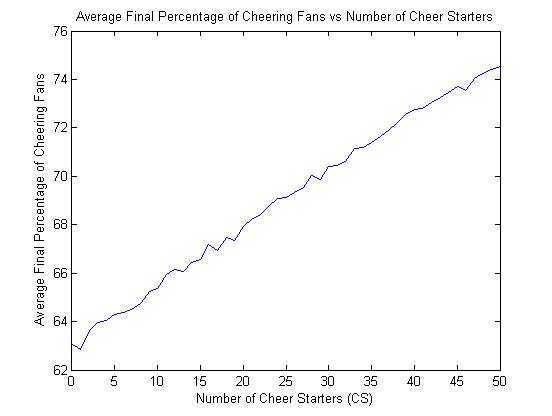
\includegraphics [width=4in] {46(1).jpg}
    			\caption [Plot of Average Final Percentage of Cheering Fans for Various Numbers of Cheer Starters] {Average final percentage of cheering fans over 1000 trials for various $CS$ values.}
    			\label{finalpercentagegraph}
    		\end{center}
\end {figure}	

\begin{table}[h!]
\begin{center}
\begin{footnotesize}\begin{tabular}{|p{5cm}|c|c|c|c|c|c|}
\hline
\textbf{Number of Cheer Starters}&0&10&20&30&39&50\\\hline
\textbf{Average Final Percentage of Cheering Fans}&63.069&65.346&67.919&70.409&72.533&74.544\\\hline
\textbf{P-value}&0.5&0.34413&0.19637&0.097951&0.047687&0.021585\\\hline
\end{tabular}
\end{footnotesize}
\caption{Average final percentage of cheering fans for various $CS$ values.}
\label{finalpercenttable}
\end{center}
\end{table}

Based on Figure \ref{finalpercentagegraph}, we can observe an approximate positive linear relationship between the average final percentage of cheering fans and the number of cheer starters. Put more succintly, as the number of cheer starters was increased, a greater number of people in the crowd ended up cheering. This positive relationship was expected, since if there are more cheer starters in the crowd urging people to cheer, more people should join the cheering. Thus this aspect of our model is consistent with reality. 
\paragraph{39 or More Cheer Starters Produce Statistically Significant Increases in Cheering }
\paragraph{}
In addition, we also observed that the p-value of the t-test comparing the average final percentage of cheering fans with $CS$ cheer starters to the average final percentage of cheering fans with 0 cheer starters decreased as $CS$ was increased. This can be clearly seen in Table \ref{finalpercenttable} which shows the p-value of the t-test for various $CS$ values. This observation can be explained by considering the postive relationship between average final percentage of cheering fans and the number of cheer starters that was previously detailed. As the number of cheer starters increases, the average final percentage of cheering fans increases as well and thus the percentage of cheering fans becomes more significant as compared to when there are 0 cheer starters. Our analysis revealed that $CS=39$ is the first $CS$ value that produces a statistically significant increase in cheering, meaning that the p-value is less than 5\% ($p=0.047$ when $CS=39$, see Table \ref{finalpercenttable}). Through our analysis we were also able to confirm that as the number of cheer starters was increased past 39, the p-values continued decreasing. This trend is shown in Table \ref{finalpercenttable} where we see that when $CS=50$, the p-value has dropped to $p=0.02$ from $p=0.047$ when $CS=39$. Based on these observations, we can conclude that when $CS\geq39$, there is a statistically significant increase in cheering after 10 rounds have passed. It is also important to note that 39 is only approximately 2\% of the total crowd (2000 people), so it would be realistic to implement this number of cheer starters in a real crowd of fans. 

\begin{figure}[h!]
    		\begin{center}
    		  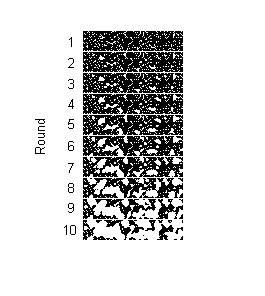
\includegraphics [width=2.5in] {n=0,46.jpg}
    			\caption [Pictorial Representation of Cheering Over Time with 0 Cheer Starters] {Cheering over time when $CS=0$. White indicates cheering.}
    			\label{cs0hist}
    			\end{center}
 \end{figure}
 
 \begin{figure} [h!]
    		\begin{center}
    			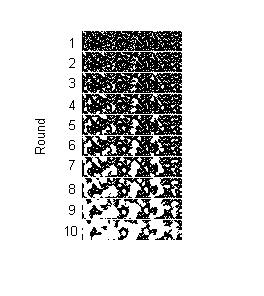
\includegraphics [width=2.5in] {n=39,46.jpg}
    			\caption [Pictorial Representation of Cheering Over Time with 39 Cheer Starters] {Cheering over time when $CS=39$. White indicates cheering.}
    		\label{cs39hist}
    		\end{center}
 \end {figure}	

\paragraph{}
Based on Table \ref{finalpercenttable} we see that there is approximately a 10\% difference in the average final percentage of cheering fans between when there are 0 cheer starters and when there are 39 cheer starters ($63.1\%$ vs $72.5\%$). Figure \ref{cs0hist} and Figure \ref{cs39hist} show a visual representation of how cheering in a crowd progresses over 10 round when there are 0 and 39 cheer starters, respectively. In these figures, white indicates cheering. There is an approximate 10\% difference in white between the two figures in round 10 that corresponds to the 10\% difference in cheering. (Note: These plots are of single trials and not averaged over 1000 trials)

\paragraph{The Rate at Which Cheering Increases Grows with the Number of Cheer Starters}
\paragraph{}
After determining the minimal $CS$ value at which there is a statistically significant increase in cheering, we focused our analysis on the effect of cheer starters on the rate at which cheering increases. A detailed examination of the percentage of the crowd cheering in each round for each $CS$ value between 1 to 50 revealed that as the number of cheer starters is increased, the rate at which cheering increases also increases. This result is shown in Figure \ref{varcsgraph}, which shows the percent of the crowd cheering in each round for several $CS$ values, and Table \ref{varcstable}, which shows values obtained from Figure \ref{varcsgraph}. Note that the data in Figure \ref{varcsgraph} and Table \ref{varcstable} is averaged across 1000 trials for each CS value. 

\begin{figure} [h!]
		\begin{center}
    			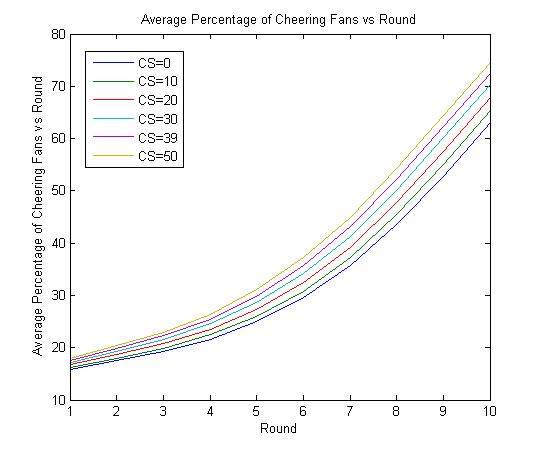
\includegraphics [width=4in] {46(2).jpg}
    			\caption [Plot of Percentage of Cheering Fans Over Time for Various Number of Cheer Starters] {The percentage of cheering fans over time for various $CS$ values.}
    			\label{varcsgraph}
    		\end{center}
\end {figure}

\begin{table}[h!]
\begin{center}
	\begin{small}\begin{tabular}{|l|c|c|c|c|}
\hline
\textbf{Round}&1&3&7&10\\\hline
\textbf{CS=0}&15.875&19.285&35.67&63.069\\\hline
\textbf{CS=10}&16.266&19.936&37.307&65.346\\\hline
\textbf{CS=20}&16.686&20.717&39.246&67.919\\\hline
\textbf{CS=30}&17.13&21.53&41.284&70.409\\\hline
\textbf{CS=39}&17.519&22.261&43.088&72.533\\\hline
\textbf{CS=50}&17.908&23.002&44.936&74.544\\\hline
\end{tabular}
\end{small}
\end{center}
\caption{The percentage of cheering fans over time for various $CS$ values.}
\label{varcstable}
\end{table}
	
\paragraph{}
Based on Figure \ref{varcsgraph} we can see that, regardless of the $CS$ value, all the trajectories of the plots have an exponential-like growth rate. However, trajectories with greater $CS$ values have a steeper slope meaning a greater rate of increase in cheering. Thus this indicates that the more cheer starters present in the crowd, the greater the rate at which cheering increases. Additionally, we also noticed that for all $CS$ values, the rate at which cheering increases (i.e.~the slope of the ploted trajectories) is greatest for later rounds. This can be easily seen in Figure \ref{varcsgraph}. For a more concrete example consider $CS=39$ in Table \ref{varcstable}. The increase in cheering between rounds 1 and 3 is $22.2\%-17.5\%=4.7\%$, or approximately an average increase of $4.7\%/2=2.35\%$ per round over 2 rounds. The increase in cheering between rounds 7 and 10 is $72.5\%-43.1\%=29.4\%$, or approximately an average increase of $29.4\%/3=9.8\%$ per round over 3 rounds. Thus rounds 7-10 have an approximate 5 times greater average percent increase in cheering as compared to rounds 1-3. 
\paragraph{}
Based on our observations above, our model suggests two conclusions: the rate at which cheering increases is positively related to the number of cheer starters, and also that the rate at which cheering increases grows as more time has passed and more people have started cheering. These results are consistent with what we would expect in reality, which are that, placing more cheer starters in a crowd should increase the growth rate of cheering, and that as more time passes, and more fans have started cheering, a greater proportion of the remaining non-cheering fans will start cheering, resulting in a greater rate of increase of cheering as time progresses.

\ifthenelse{\boolean{@twoside}}{\myclearpage}{}
\prefacesection{Conclusion}
\paragraph{}
After extensive analysis using this model, we can safely conclude that this model is reasonably qualitalively accurate; it follows realistic assumptions and the results of this model are consistent with what we would expect to observe in reality. Based on the simualtion results of our model we can recommend to BJU that cheer starters are in fact effective at increasing the amount of cheering in a crowd at sporting events. 
\paragraph{}
After simulating a crowd of 2000 fans in a rectangular-shaped section of bleachers similar in shape to the home team bleachers of Homewood Field, we found that 39 randomly placed cheer starters (or approximately 2\% of the total crowd) is enough to generate a statistically significant increase in cheering. Furthermore, there exists a positive relationship between the final percentage of the crowd cheering and the number cheer starters. As the number of cheer starters grows, the final percentage of the crowd which is cheering increases as well. Increasing the number of cheer starters past 39, results in even greater percentages of cheering fans.
\paragraph{}
Another key observation we made based on our model were that the rate at which cheering increases is also postively related to the number of cheer starters. As we increased the number of cheer starters, we found that the rate at which cheering increased also increased. One other important observation we noticed based on our model was the rate at which cheering increases grows as more time progresses and more people have begun cheering. Regardless of how many cheer starters were placed in the crowd, the rate at which cheering increased was always greater for later time points and when more people had begun cheering.
\paragraph{}
Based on the conclusions drawn from our model, we recommend to BJU to initially place 80 cheer starters randomly in the 4000 seat capacity home team bleachers at Homewood Field during sporting events and see if there is a noticeable increase increase in cheering. Eighty cheer starters is 2\% of the total capacity of the bleachers and thus is a logical number of cheer starters to initially try based on our results. Furthermore, 80 cheer starters is not an unreasonable number of students to recruit for the job. If BJU is not satisfied with the increase in cheering and wants a greater increase, or if they want to increase the growth rate of cheering so that fans in the crowd begin cheering sooner, our model suggests that they can try greater numbers of cheer starters. Additionally, if BJU has computers with enough computational power, they can use our model and simulate a crowd of 4000 fans and see what our model predicts as the minimal number of cheer starters to generate a statistically significant increase in cheering. BJU could also then use the 4000 fan model to determine how many cheer starters are required to increase cheering to a level that is desired by them. 
\paragraph{}
At this stage, our model at this stage is reasonably qualitatively accurate. However, if our model is found to be inaccurate after re-conciling it with real data, it will need to be further refined. This is a process that all models must undergo; even reasonably accurate models can be made more accurate. We recommend to BJU that they attempt to measure the percentage of fans cheering at real sporting events. This data can then be used to further fine-tune the model parameter values and thus improve the model.    
\paragraph{}   
We believe that our stochastic model will be viable for the future, and will serve as a framework for future research into sociodynamic studies. Ideally, this model can be applied to almost all settings with audiences or crowds, and can be used to influence the audience or crowd to actively acquiesce to an opinion or action. We believe that this model will propel our knowledge of sociodynamic settings, and future improvements to our model will allow for even more accurate predictions of crowd behavior. 
%\paragraph{}
%The goals of this project have been accomplished and the deliverables have produced in a timely fashion. The following list summarizes our goals and objectives in a clear and concise manner:
%		\begin{itemize}
%			\item Provide BJU with a simple model of fan participation in cheering at Homewood Field,
%			\item Provide simulation results from the model which determine if cheer starters are effective in increasing cheering,
%		\end{itemize}
%\paragraph{Deliverables}
%	\begin {itemize}
%	\item MATLAB R2009b and R combination package with test scripts that can be used to reproduce our numerical and simulation test results
%	\item Technical report and presentations summarizing the work
%	\end{itemize}
 

%\ifthenelse{\boolean{@twoside}}{\myclearpage}{}
%\prefacesection{Remaining Work to Be Done}
%\paragraph{}
%For our current model, we picked sample parameters for purposes of demonstration so far. For example, our initial threshold is 11 (one standard deviation above the normal distribution centered at 10), and the absolute threshold was 45 or 50. The simulation ran for 10 rounds for a crowd of 2,000 people ($20$ x $100$ sized matrices). However, we have not yet determined an finalized set of model parameters for the entire project. For the remaining time we have to work on this project, we must pick a definitive initial threshold, absolute threshold, size of the crowd (i.e.~$n$ and $m$), and number of total rounds.
%\paragraph{}
%We must also investigate the effect of cheer starters on the percentage of fans cheering in the final round. Our current model does not take into account cheer starters; rather, it simulates a stochastic, general crowd susceptible to the influence of people cheering around them. Once all the parameters are finalized (including the number of cheer starters), we plan to randomly place the cheer starters within the crowd. We can then use Monte Carlo simulations to repeatedly run our model to determine the average percentage of fans cheering at the end of the final round when there are no cheer starters and also the percentage when there are cheer starters randomly placed in the crowd. If the final cheering percentage is statistically significantly greater with cheer starters then without, it would demonstrate that cheer starters are effective in increasing cheering. 
% 
%\paragraph{}
%If time permits, we could also add a function to our model which allows us to manually dictate where the cheer starters are placed. This would allow us to try and find patterns in cheer starter placements which maximize cheering. Right now, we hypothesize certain patterns will produce a larger percentage of overall people cheering than other patterns.
%
%\paragraph{}
%Finally, we can complete the project by polishing the code in MATLAB and writing R documentation for a MATLAB coded-R documented package. We will also need to write a final report and give a final presentation.
%\include{D_Analysis}
%\include{E_Results}
%\include{F_Conclusion}

%\include{chapter1}
%\include{chapter2}
%\include{chapter3}
%\include{chapter4}
%\include{chapter5}
%\include{chapter6}


\appendix
\ifthenelse{\boolean{@twoside}}{\myclearpage}{}
\prefacesection{Glossary}

%\chapter{Lemmas}\label{Lemma}

%\chapter{Glossary}\label{Glossary}

%\vspace{12pt} 

\vspace{8pt} \noindent {\bf Cheering}. Any action performed by a fan which shows support for a sports team. Examples include chanting the school fight song, waving a rally towel, doing the wave, or clapping in general applause.

\vspace{8pt}
\noindent {\bf Cheer Starter}. A student volunteer who leads and urges other fans around him/her to cheer.


\ifthenelse{\boolean{@twoside}}{\myclearpage}{}
\prefacesection{Abbreviations}
%\chapter{Abbreviations}\label{Abbreviations}


\noindent {\bf BJU}.  Blue Jays Unlimited

%\vspace{5pt}
%
%\noindent {\bf JHU.}  Johns Hopkins University

%\endinput

% Add your bibliography to Contents
\appendix
\ifthenelse{\boolean{@twoside}}{\myclearpage}{}
\prefacesection{Team GitHub Address}
\url{https://github.com/BJUnlimited}

\ifthenelse{\boolean{@twoside}}{\myclearpage}{\newpage}
\addtocontents {toc}{\protect \contentsline {chapter}{REFERENCES}{}}
\addcontentsline{toc}{chapter}{Selected Bibliography Including Cited Works}  

% Bibliography must come last.
\bibliographystyle{unsrt}
\renewcommand\bibname{Selected Bibliography Including Cited Works}
%\nocite{*}  % List ALL references in your references, not just the ones cited in the text.
% This scheme automatically alphabetizes the Bibliography.
\bibliography{extra/biblioWS}
\end{document}
